\documentclass[conference]{IEEEtran}
\IEEEoverridecommandlockouts
% The preceding line is only needed to identify funding in the first footnote. If that is unneeded, please comment it out.
\usepackage{cite}
\usepackage{amsmath,amssymb,amsfonts}
\usepackage{algorithmic}
\usepackage{graphicx}
\usepackage{textcomp}
\usepackage{xcolor}
\usepackage{parskip}
\usepackage{changepage}
\usepackage{float}
\usepackage{hyperref}
\hypersetup{colorlinks=true,urlcolor=blue}

\newenvironment{quoteindent}{\begin{adjustwidth}{0.7cm}{}}{\end{adjustwidth}}

\def\BibTeX{{\rm B\kern-.05em{\sc i\kern-.025em b}\kern-.08em
    T\kern-.1667em\lower.7ex\hbox{E}\kern-.125emX}}
\begin{document}

\title{Multithreaded Ray Tracing}

\author{\IEEEauthorblockN{Pedro Contipelli}
\and
\IEEEauthorblockN{Tanner Fleming}
\and
\IEEEauthorblockN{Christopher Gray}
\and
\IEEEauthorblockN{Gavin Gilbert}
\and
\IEEEauthorblockN{Diego Rodrigues}

}

\maketitle

%\begin{abstract}
%This document is a model and instructions for \LaTeX.
%This and the IEEEtran.cls file define the components of your paper [title, text, heads, etc.]. %*CRITICAL: Do Not Use Symbols, Special Characters, Footnotes, 
%or Math in Paper Title or Abstract.
%\end{abstract}

%\begin{IEEEkeywords}
%component, formatting, style, styling, insert
%\end{IEEEkeywords}

\begin{center}
\href{https://github.com/PedroContipelli/Parallel-Raycasting}{GitHub Repo}
\end{center}

\section{Abstract}
In this research project, we explore the problem of Multithreaded Ray tracing. Ray tracing is defined as “determining the visibility of surfaces by tracing imaginary rays of light from a viewer/camera’s eye to objects in a scene.” Usually, the idea is to cast one ray of light per pixel that is being rendered and determine which object it first intersects in a 3D scene, then calculating light bouncing effects as necessary. This allows computers to determine which parts should be shown when there are multiple different, possibly intersecting (from a 2D perspective) objects. However, since the calculation of each ray is computationally independent of one another, we believe that using concurrent programming can provide us a significant speedup by allowing us to perform ray calculations in parallel. In this paper, we show that adding both naive multi-threading and better load-balancing with thread pools can allow us to reduce our runtime significantly for complex scenes.

\section{The State of the Art in Ray-Tracing}

Ray Tracing is a very solvable problem. We have algorithms, we know it's highly parallel, we just need the computational power to pull it off. Finally, after almost 50 years after the inception of ray-tracing in the late 1970s, we’ve only just recently reached a point where real-time ray-tracing is a possibility.

Pixar's “Cars”, from 2006, became the first feature film to use ray-tracing\cite{b1}. However, it took many hours just to render a single frame of the film. To reduce computation time per frame from a scale of several hours to a scale of several milliseconds would require an advancement in computational power of over 500,000 times.

“Global Illumination” was told to be possible by NVIDIA Research as of the GTX 770 hardware (released May 30, 2013), which was less powerful than a PlayStation 4. In 2017, NVIDIA Research published a paper detailing global illumination with fully dynamic lighting, rendered in a mere 3.9ms\cite{b2}. They were using an Intel Core i7-3770k CPU with 32GB of memory and an NVIDIA Titan X Pascal GPU. A single frame generated within fractions of a second. A massive improvement compared to the days of Pixar’s “Cars”.

NVIDIA isn't the only group to be researching ray-tracing, though. Intel has been publishing papers for just as long, and had the first real-time ray-tracing demo in a game using the Quake Wars engine in September of 2009\cite{b3}. And this was running only on CPUs, with no help from a GPU.

The major hurdle for ray-tracing, even today, has been computational power. More efficient algorithms and post-processing tricks like denoising have moved the goalposts closer to us, but we still need even more computational power to realize the eventual goal: High-Quality Real-Time Ray-Tracing.

In March of 2018, NVIDIA released a video demo called "Reflections"\cite{b4}. This was intended to generate hype for their new RTX series graphics cards, but it also acted as a demonstration of some new techniques regarding sophisticated denoising and upscaling techniques. These improvements allowed for low resolution ray-tracing to appear passable to end users at playable frame-rates. 

Tim Sweeney of Epic Games and Unreal Engine:


\begin{quoteindent}
"You know, we're getting to the point now where we can render photo-realistic static scenes without humans with static lighting. Today's hardware can do that, so part of that problem is solved. Getting to the point of photo-realistic dynamic environments, especially with very advanced shading models like wet scenes, or reflective scenes, or anisotropic paint, though... maybe forty Teraflops is the level where we can achieve all of that."
\end{quoteindent}


At the time of this quote, the Titan X could give somewhere around 1/4 of that, 10 Teraflops. Nowadays, we're at approx. 23 Teraflops with the AMD Radeon RX 6900 XT at peak performance, or even a theoretical peak of 35 Teraflops with an NVIDIA GeForce RTX 3090. We have begun to reach the point where real-time ray-tracing is a reality. We've gathered enough processing power to start making it a reality. Any further improvements can now be focused on increasing quality, rather than enabling real-time computation.

\section{Methods}

\subsection{Basics of Raytracing}
\subsubsection{Creating the Image File}
To be able to develop ray tracing one must first know how to form an image, with the most straight forward way being writing to a file ppm file. A PPM file is a 24-bit color image that has been formatted as text. It assigns a number between 0 and 65536 to each pixel, indicating the pixel's color. The image height and width, as well as whitespace data and the maximum color value, are all stored in PPM files \cite{b5}. PPM files are used due to it’s lack of need to include another C++ library, as well as its ease of use. 

\subsubsection{Using vec3 Class}
Almost every graphics application has a class (or several) for storing geometric vectors and colors. These vectors are 4D in many systems (3D plus a homogeneous coordinate for geometry, and RGB plus an alpha transparency channel for colors). Three coordinates are sufficient for our needs. For colors, locations, directions, offsets, and whatever else, we'll utilize the same vec3 class. Some people object to this because it does not prevent you from doing anything ridiculous, such as changing the color of a location \cite{b6}. 

\subsubsection{Creating a ray, camera, and background}
A ray class and a computation of what color is observed along a ray are the only things that all ray tracers have in common. Consider a ray as a function \(R(t)=A+tB\). P is a three-dimensional position along a line. The ray origin is A, while the ray direction is B. The ray parameter t is a positive integer (double in the code). P(t) advances the point along the ray when a different t is entered. You can move anywhere on the 3D line if you use negative t values. For positive t, you only get the bits in front of A, which is known as a half-line or ray\cite{b6}.

\begin{figure}[h]
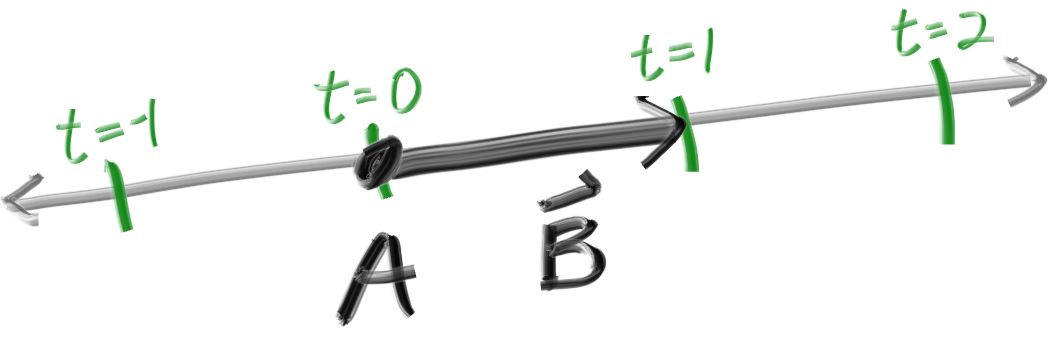
\includegraphics[width=8cm]{images/ch4-1.jpg}
\centering
\end{figure}

The ray tracer's basic function is to transmit rays through pixels and compute the color perceived in their direction. (1) calculate the ray from the eye to the pixel, (2) determine which objects the ray contacts, and (3) compute a color for that intersection point are the processes involved. When I initially start working on a ray tracer, I always start with a simple camera to get the code running. In addition, I create a basic ray color(ray) method that returns the backdrop color\cite{b6}.

A virtual viewport through which our scene rays can pass in addition to the pixel measurements for the generated image is needed. The aspect ratio of the viewport should be the same as our produced image for the usual square pixel spacing. The distance between the projection plane and the projection point should also be set to one unit. This is known as the "focal length," which should not be confused with the "focus distance".

The camera, or view, should be placed at the center of image and interpreted as such.

\begin{figure}[h]
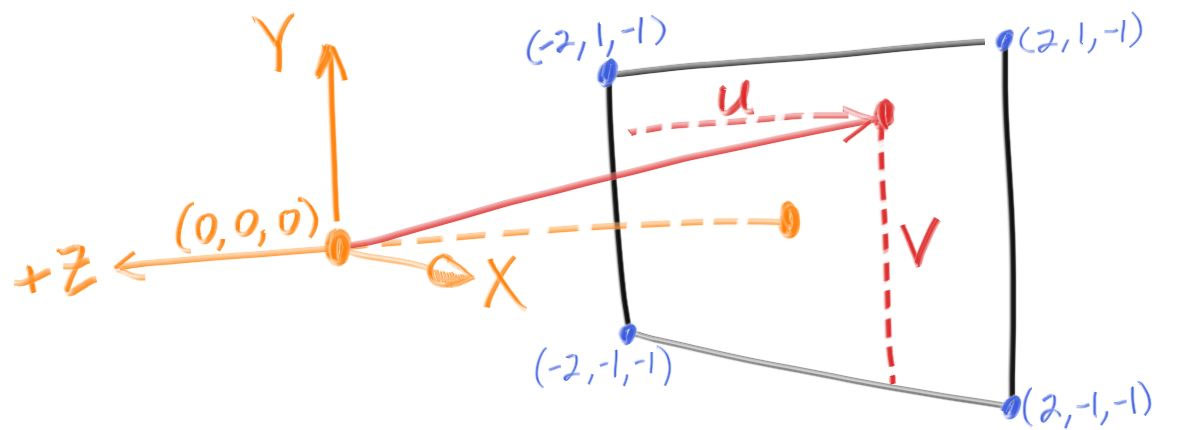
\includegraphics[width=6cm]{images/ch4-2.jpg}
\centering
\end{figure}

\subsubsection{Creating a Sphere}
Recall the equations of a sphere
\begin{align*}
x^2+y^2+z^2 &= R
\end{align*}
where points inside the sphere are where 
\begin{align*}
x^2+y^2+z^2 &> R
\end{align*}
If the sphere is centered at \((C_x, C_y, C_z)\) then it can be represented by 
\begin{align*}
(x-C_x)^2+(y-C_y)^2+(z-C_z)^2&=r^2
\end{align*}

Vector \(P=(x,y,z)\) can be denoted from the center by \((P-C)\) then
\begin{align*}
(P-C)\times(P-C)&=(x-C_x)^2+(y-C_y)^2+(z-C_z)^2=r^2
\end{align*}
We want to know if our ray \(P(t)=A+tb\) ever collides with the sphere. If it collides with the sphere, P(t) fulfills the sphere equation for some t. As a result, we're looking for any t in which this is true:
\begin{align*}
(A+tb-C)\times(A+tb-C)&=r^2
\end{align*}
That can then be expanded to
\begin{align*}
t^2b\times b+2tb\times(A-C)+(A-C)\times(A-C)-r^2&=0
\end{align*}
When you solve for t, you'll get a square root portion that's either positive (indicating there are two actual solutions), negative (meaning there are no real solutions), or zero (meaning one real solution). In graphics, algebra nearly always has a direct relationship with geometry. We have the following:
\begin{figure}[h]
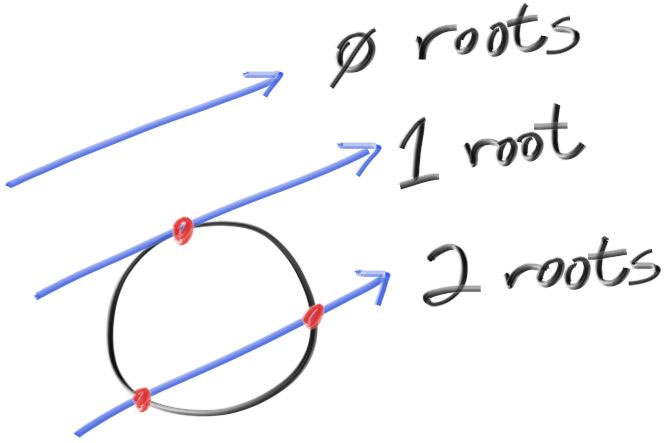
\includegraphics[width=3cm]{images/ch4-3.jpg}
\centering
\end{figure}
Normals' second design decision is whether or not they should constantly point out. Currently, the found normal will always be in the direction of the intersection point (the normal points out). The normal points against the beam if it intersects the sphere from the outside. The normal (which always points out) points with the beam if it intersects the sphere from the inside. Alternatively, the normal can always point away from the ray. The normal will point outward if the ray is outside the sphere, but it will point inward if the beam is inside the sphere.

\subsubsection{Surface Normals and Multiple Objects}
The surface normal is a vector that is perpendicular to the surface at the point of intersection. For normals, there are two design considerations to make. One consideration is whether or not these normals are of unit length. The outer normal for a sphere is in the direction of the impact point minus the center:
\begin{figure}[h]
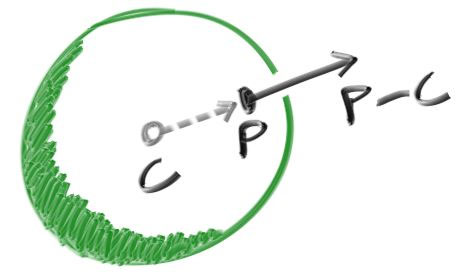
\includegraphics[width=6cm]{images/ch6-1.jpg}
\centering
\end{figure}
\subsubsection{Front Faces Versus Back Faces}
Normals' second design decision is whether or not they should constantly point out. Currently, the found normal will always be in the direction of the intersection point (the normal points out). The normal points against the beam if it intersects the sphere from the outside. The normal (which always points out) points with the beam if it intersects the sphere from the inside. Alternatively, the normal can always point away from the ray. The normal will point outward if the ray is outside the sphere, but it will point inward if the beam is inside the sphere.
\begin{figure}[h]
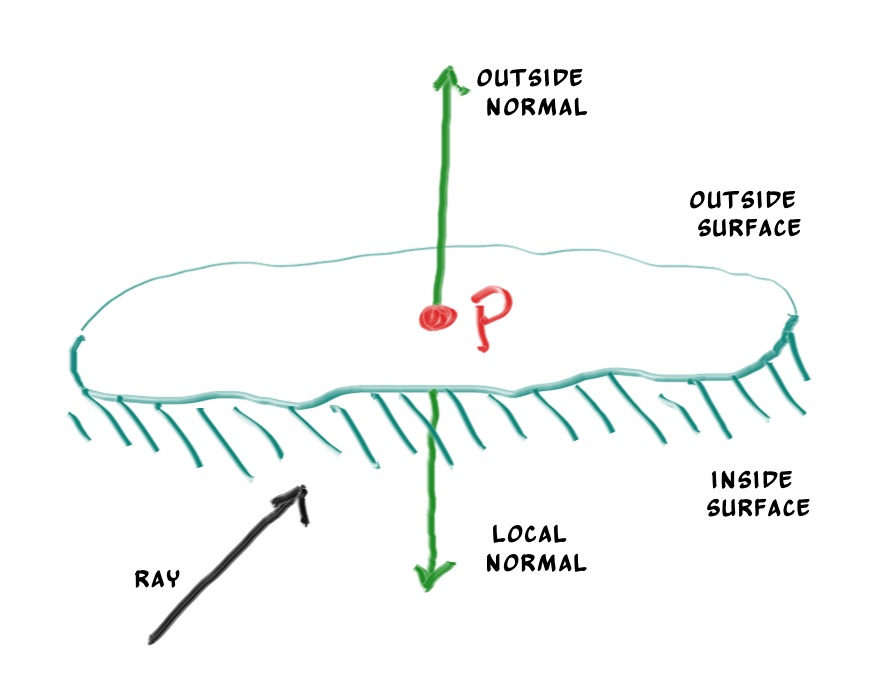
\includegraphics[width=6cm]{images/ch6-2.jpg}
\centering
\end{figure}
\subsubsection{Front Faces Versus Back Faces}
Because the edge pixels are a blend of some foreground and some background, there are normally no jaggies along edges when a camera produces an image. The similar effect can be achieved by averaging a number of samples within each pixel. 

We have many samples within a pixel and transmit rays through each of them for a given pixel. After that, the colors of these rays are averaged:
\begin{figure}[h]
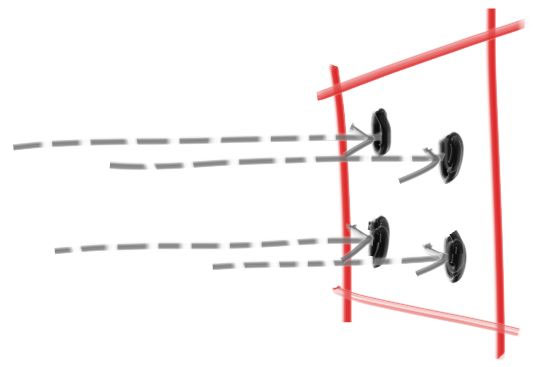
\includegraphics[width=6cm]{images/ch7.jpg}
\centering
\end{figure}

\subsection{Advanced Raytracing}
One design decision is to separate materials from geometry. Light can be either reflected, refracted, or absorbed. A simple diffuse object randomizes the direction of light that reflects off of its surface. And absorbs light according to how “dark” its surface is.

Our algorithm for generating a random diffuse bounce ray in order to calculate reflected light is as following:
\begin{enumerate}
  \item Find the tangent unit radius sphere on the same side as the ray origin.
  \item Pick a random point $S$ inside this sphere using rejection sampling
  \begin{enumerate}
      \item Pick a random point in the unit cube ($-1 <= x,y,z <= 1$)
      \item Reject and try again if not in sphere.
  \end{enumerate}
  \item Send a ray from the hit point $P$ to $S$. This is the reflected light vector $S - P$
\end{enumerate}

Because our function for determining a ray’s color recursively calls itself until the light stops bouncing (which may take a long time), we must limit its maximum recursion depth by returning no light contribution at the max.

\begin{figure}[h]
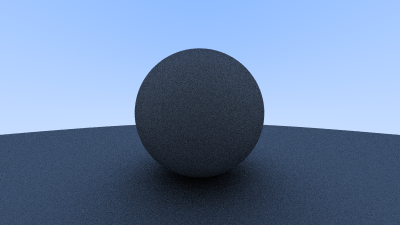
\includegraphics[width=7cm]{images/diffuse_sphere.png}
\centering
\end{figure}

We also gamma-correct the image by applying $sqrt()$ to the $R,G,B$ values to get:

\begin{figure}[h]
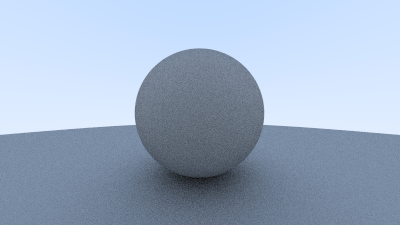
\includegraphics[width=7cm]{images/gamma-correction.png}
\centering
\end{figure}

Another design decision is to create an abstract class for materials. Every material should:
Produce a scattered ray (or absorb the incident ray). And if scattered, define behavior and light reduction factor

When working with smooth metals, we want our ray to reflect rather than scatter.

\begin{figure}[h]
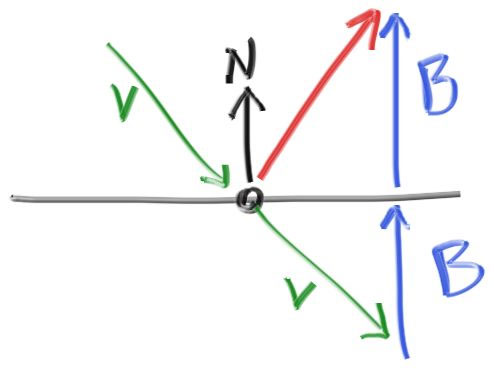
\includegraphics[width=5.5cm]{images/reflect_vector.jpg}\\
Reflected Vector (red): $v - 2(v \cdot n)n$
\centering
\end{figure}

\begin{figure}[h]
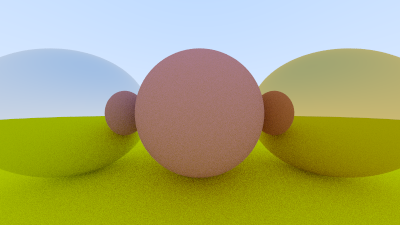
\includegraphics[width=6cm]{images/metal_shiny.png}\\
Rendering with smooth (direct) reflections
\centering
\end{figure}

However, since smooth metals are not perfect mirrors, we add in a fuzziness parameter to make things look more realistic, which perturbs the reflection ray slightly.

\begin{figure}[h]
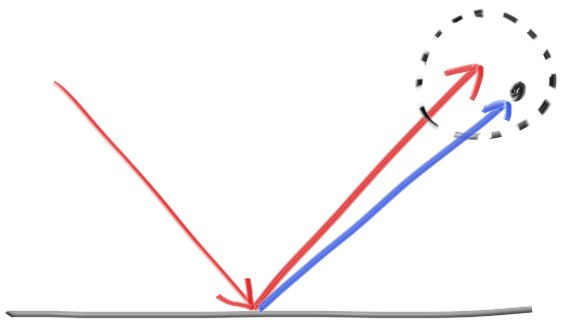
\includegraphics[width=6cm]{images/reflect_fuzzy.jpg}
\centering
\end{figure}

\begin{figure}[h]
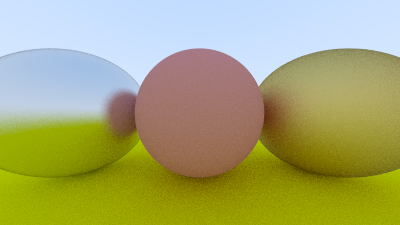
\includegraphics[width=6cm]{images/metal_fuzzy.png}\\
Rendering with fuzziness
\centering
\end{figure}

Dielectrics or clear materials such as water, glass, and diamonds behave a bit differently. When a light ray hits a dielectrics’ surface, it splits into one reflected ray and one refracted ray. To keep things simple, we will simply randomly choose one of the rays to calculate for each interaction.

Refracted rays can be calculated with a physics principle known as Snell’s Law:
\[ \eta \cdot sin(\theta) = \eta' \cdot sin(\theta') \]

Here, $\theta$ is angle from the normal, and $\eta$ is the refractive index (constant for each material). Note: when there is no solution for $\theta'$, that means the ray must reflect.

The last key feature of any sophisticated raytracer would be the ability to position and orient the camera anywhere in the space of your coordinate system.

\begin{figure}[H]
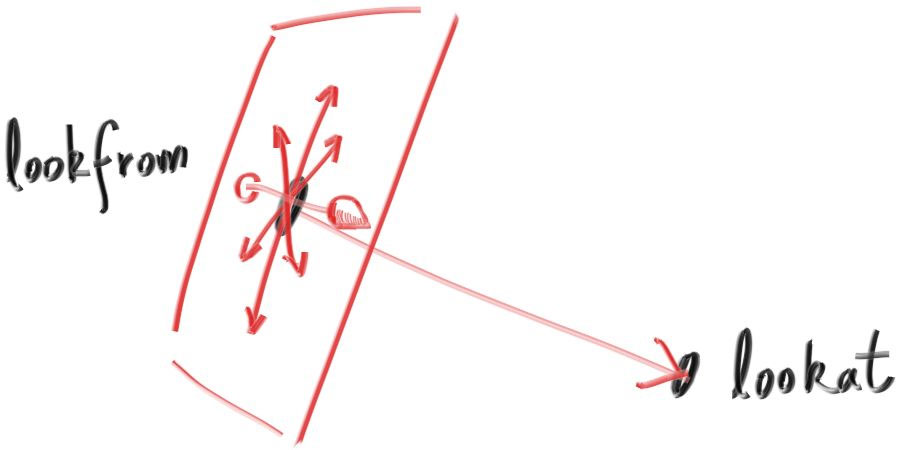
\includegraphics[width=4cm]{images/camera1.jpg}
\centering
\end{figure}

This is something we accomplish by specifying 2 points: "lookfrom" and "lookat" which form a vector that gives us the direction the camera will be pointed. Then generating 2 more vectors via arbitrarily picking a vector $vup = (0,1,0)$ and taking cross-products in order to form a complete orthonormal basis which also encodes the "roll" or sideways rotation of the camera in addition to its viewing direction.

\begin{figure}[h]
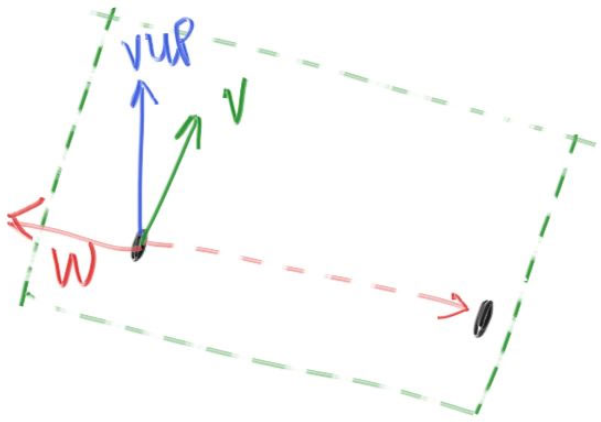
\includegraphics[width=5cm]{images/camera2.png}\\
\centering
\end{figure}

Now, we can arbitrarily position the camera to view the scene from any angle:

\begin{figure}[H]
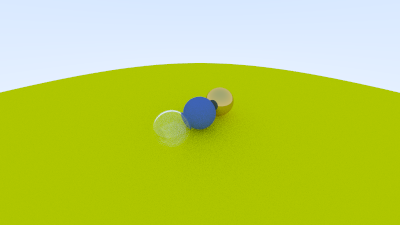
\includegraphics[width=6cm]{images/camera3.png}
\centering
\end{figure}

\begin{figure}[H]
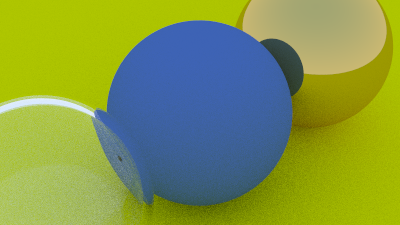
\includegraphics[width=6cm]{images/camera4.png}
\centering
\end{figure}

\subsection{Our Implementation}

We broke up our implementation into several header files that hold the various functions required to compute the ray-tracing algorithm. We did this to keep our main file more organized and to make it easier to implement multi threading.
\begin{figure}[H]
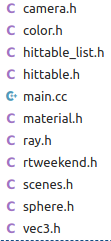
\includegraphics[width=4cm]{images/fileStructure.png}\\
File Structure
\centering
\end{figure}
Most of the files are straight forward. 
\begin{itemize}
    \item \textbf{camera.h} holds the implementation of a virtual camera class.
    \item  \textbf{color.h} holds two functions that output the RGB values of an input pixel color.
    \item  \textbf{hittable\_list.h} holds a class that is an abstraction of all the objects a ray can intersect with.
    \item  \textbf{hittable.h} class that holds a function to take in a ray and compute anything it might hit.
    \item  \textbf{material.h} class that holds different material types an item can have.
    \item  \textbf{ray.h} holds the ray class that computes the rays.
    \item  \textbf{rtweekend.h} this is our main header file that holds many of our basic math functions.
    \item  \textbf{scenes.h} contains the code for generating the custom scenes rendered.
    \item  \textbf{sphere.h} implementation of the hittable class in the shape of a sphere.
    \item  \textbf{vec3.h} As mentioned earlier this is our class for storing geometric vectors and colors.
\end{itemize}
\textbf{main.cc:} This is where the magic happens. This is where the scene gets rendered. This is also where we implemented multi-threading. In this file we have declared 3 helper functions. 
\begin{itemize}
    \item \textbf{ray\_color} this function takes in a ray, the hittables, and depth then returns the color vector.
    \item \textbf{random\_scene} Generates a random scene for the program to render.
    \item \textbf{render} this function takes in the start and end pixels, output stream, image height and width, samples per pixel, max depth, virtual camera, and the world to be rendered. Then renders it.
\end{itemize}

\subsection{Parallelization}

\subsubsection{Naive}
Our first rudimentary attempt at implementing multithreading involves simply dividing our image into groups of scanlines, and assigning one thread to compute each group. Then, once all threads have completed, we join it all together into one image. Note: this does not consider load balancing at all. However, even with this simple implementation we are able to reduce our render time for our final image from $88.98$ to $20.66$ minutes.

\subsubsection{Thread Pools}
Our second attempt at this problem we implemented thread pooling in an attempt to have threads spend less time idling and more time getting work done. Our thread pool implementation works by making a thread pool that creates n number of threads. These threads are then added to a work function that continuously try's to dequeue a task from the task queue. The task queue is a concurrent queue that uses a spin lock. Then endWhenEmpty function is called on the threads and joins all threads when the task queue is empty.

\subsection{Experiments}

\begin{figure}[H]
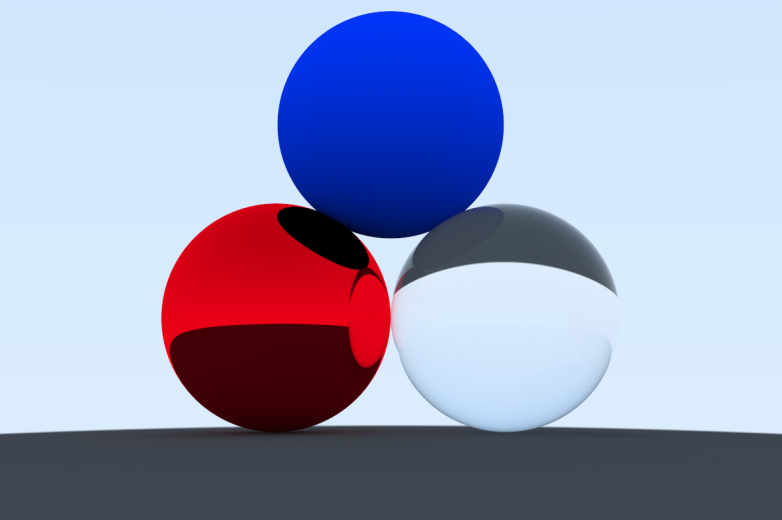
\includegraphics[width=6cm]{images/Scene1.png}
\centering\\
Fig. 1
\end{figure}

\begin{figure}[H]
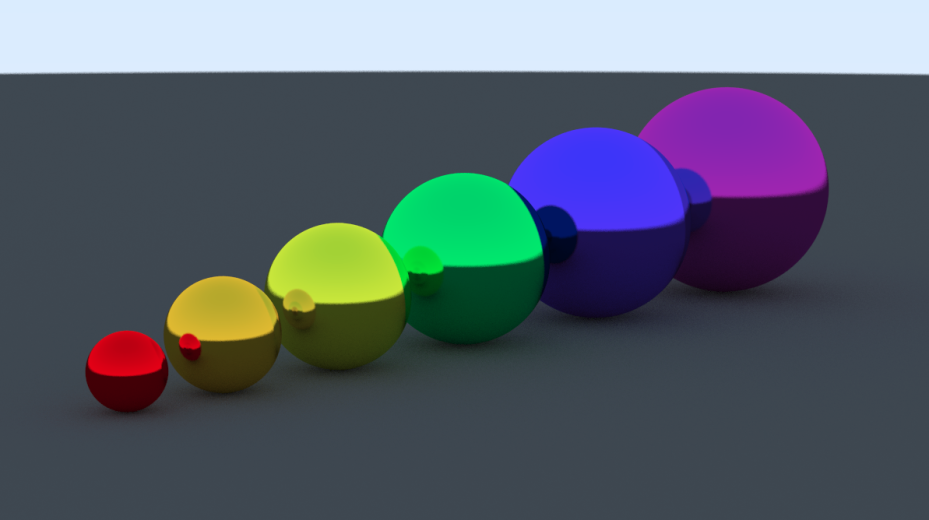
\includegraphics[width=6cm]{images/Scene3.png}
\centering\\
Fig. 2
\end{figure}

\begin{figure}[H]
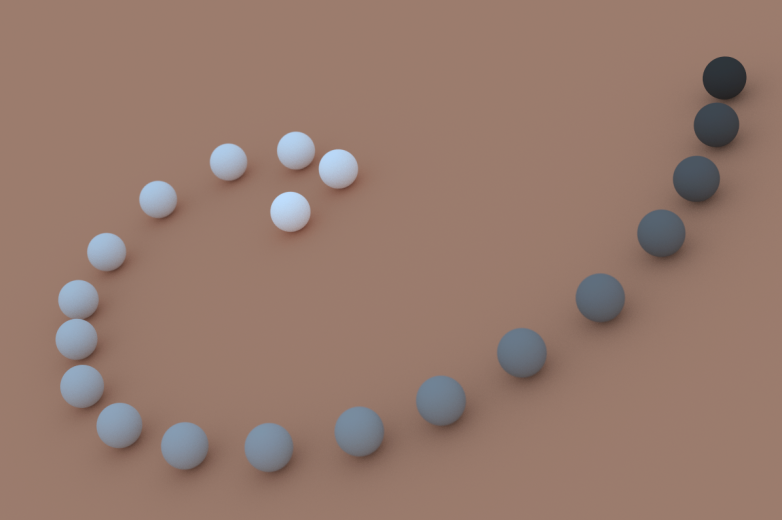
\includegraphics[width=6cm]{images/Scene4.png}
\centering\\
Fig. 3
\end{figure}

\begin{figure}[H]
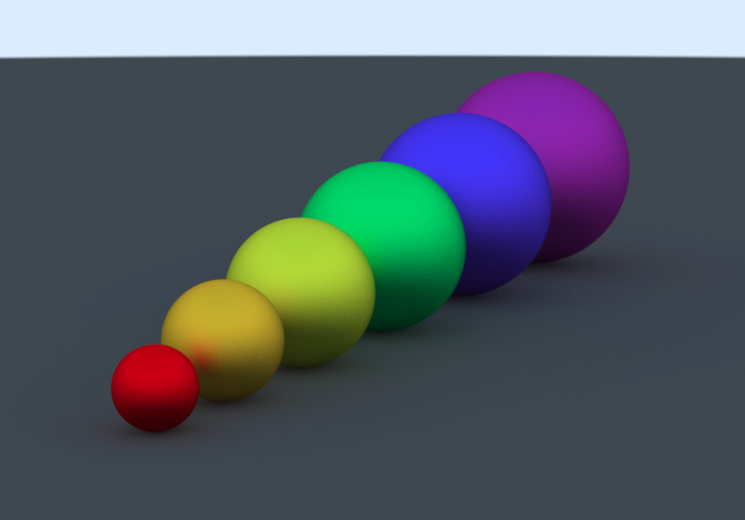
\includegraphics[width=6cm]{images/Scene2.png}
\centering\\
Fig. 4
\end{figure}

\begin{figure}[H]
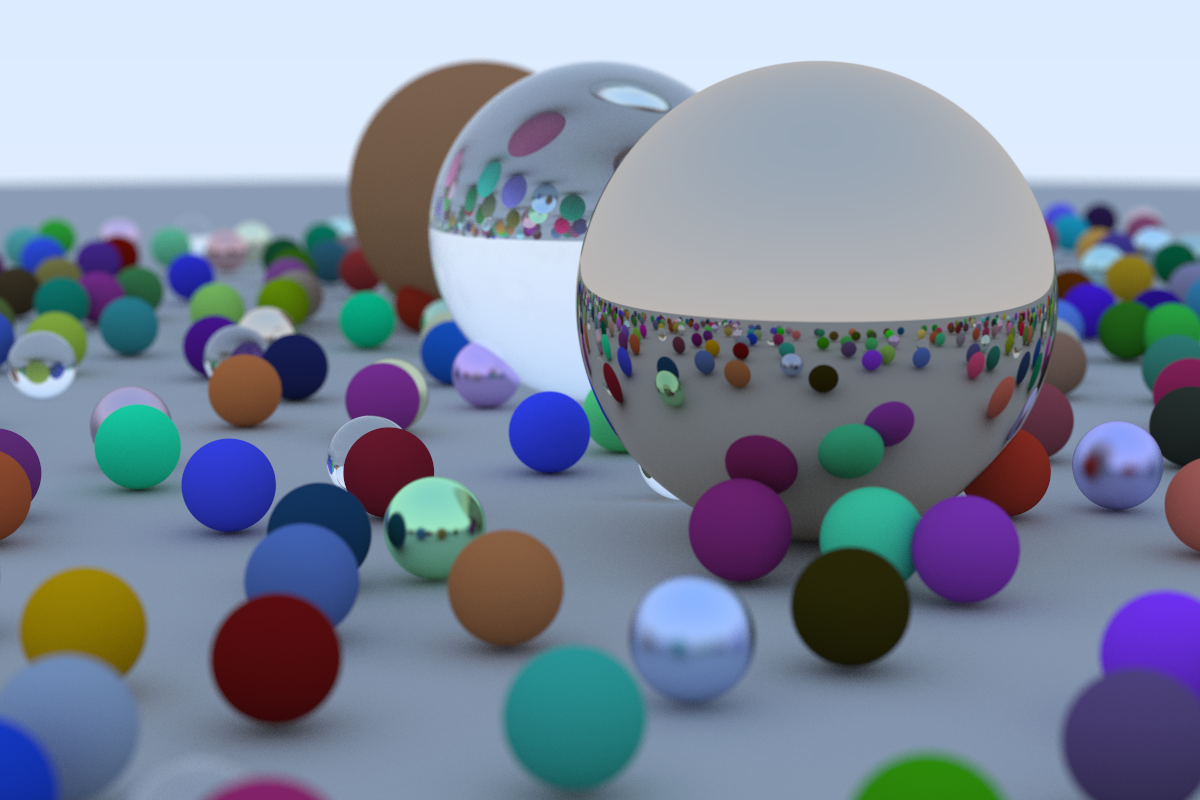
\includegraphics[width=6cm]{images/FinalRender.png}
\centering\\
Fig. 5
\end{figure}

\begin{center}
\begin{tabular}{||c c c c||} 
 \hline
  & Fig. 1  & Fig. 2 & Fig. 3 \\ [0.5ex] 
 \hline\hline
 Single-threaded & 208s & 308s & 532s \\ 
 \hline
 Naive Multithreading & 330s & 453s & 488s \\
 \hline
 Thread Pools & 353s & 482s & 511s \\
 \hline
\end{tabular}
\end{center}

\section{Discussion/Conclusion}
We noticed after testing and tabulating the runtimes for rendering the simpler scenes (figures 1 and 2 for example) that unfortunately runtime can increase after implementing multithreading for scenes with fewer objects. This occurs, we believe, due to the overhead associated with creating and running several threads being larger than the actual time it saves to use them. However for figure 3 which contains more objects, we noticed that our naive multithreading solution was able to render the scene faster as the actual processing for the render is more intensive than the overhead necessary.

We ended up implementing thread pools from scratch in the end, but it seems that the required overhead makes it consistently slower than explicit multi-threading for our small-scale tests. We believe that if tested with larger-scale scenes (more objects to calculate intersection), that the overhead required would be outweighed by the benefit of distributing the workload evenly among all threads. Another explanation for the slowness could be that the concurrent-queue that we used to manage jobs was not wait-free, so it's possible that it caused some hang-ups when multiple threads tried to access the jobs at the same time.

\section{Appendix}
\subsection{Challenges}\label{AA}
One of the main problems we faced when beginning the implementation of parallelization with ray-tracing was evenly distributing tasks between threads. C++ does not have thread pools built-in. Thread pools would help in the organization of the threads to prevent idle threads from being useless. Our current implementation evenly splits the threads and waits for all to complete and does not consider load balancing. Another challenge we foresaw from the beginning is several of the research articles mentioning the difficulty of a multithreading implementation for ray-tracing. This did not stop us. After the initial implementation of the code gathered from our resources we had a discouraging runtime of 8 hours. After this initial runtime, we realized we had a lot of work ahead to get a useful implementation.
\subsection{Completed Tasks}\label{AA}
We have researched ray tracing and its applications. Studying different implementations and best practices for the technique. We followed a coding course that implemented a single-threaded implementation of the ray-tracing algorithms we were studying. Then we researched the specific conversions we would need to make to parallelize it. We implemented a basic version of parallelization in the ray-tracing code and saw a significant decrease in total runtime for larger and more complex scenes. After further tweaks to this code, we were able to get this number even lower by making the targets more reasonable. We also implemented thread pools using a concurrent queue to try and introduce load-balancing.

\subsection{Remaining Tasks}\label{AA}
If we were to continue this project, there would probably be 2 things we could do. 1) We could build larger test scenes for the algorithm to render. This would allow us to test the effect that larger and higher-quality scenes have on rendering time based on which algorithm is being used, rather than simply assuming based on small-scale findings. 2) We could introduce a better load-balancing algorithm into the mix, such as maybe implementing thread pools with a wait-free concurrent queue, while still making sure that each thread is doing the same amount of work. We believe this could lead to more overhead, but also lead to higher performance and faster rendering for the aforementioned larger test cases.

\begin{thebibliography}{00}
\bibitem{b1} P. Christensen, J. Fong, D. Laur and D. Batali, "Ray Tracing for the Movie 'Cars'", IEEE, 2006.
\bibitem{b2} A. Silvennoinen and J. Lehtinen, "Real-time Global Illumination by Precomputed Local Reconstruction from Sparse Radiance Probes", Association for Computing Machinery, 2017.
\bibitem{b3} C. Kowaliski, "Intel shows Larrabee doing real-time ray tracing", The Tech Report, 2009. [Online]. Available: https://techreport.com/news/17641/intel-shows-larrabee-doing-real-time-ray-tracing/.
\bibitem{b4} “Reflections” – A Star Wars UE4 Real-Time Ray Tracing Cinematic Demo. ILMxLAB, 2018.
\bibitem{b5} “Portable Pixmap Image File,” Fileinfo.com, 2020.
\bibitem{b6} Github.io, 2020. https://raytracing.github.io/books/RayTracingInOneWeekend.html (accessed Mar. 25, 2022).
\end{thebibliography}

\end{document}
